\documentclass[a4paper,10pt]{article}

\usepackage[T1]{fontenc}
\usepackage[utf8]{inputenc}
\usepackage{graphicx}
\usepackage{xcolor}
\usepackage{fourier}
\usepackage{caption}
\usepackage{subcaption}
\usepackage{cprotect}

\usepackage{tgtermes}

\usepackage[
pdftitle={Statistical Machine Learning}, 
pdfauthor={Inez Wijnands \& Guido Zuidhof, Radboud University Nijmegen},
colorlinks=true,linkcolor=blue,urlcolor=blue,citecolor=blue,bookmarks=true,
bookmarksopenlevel=2]{hyperref}
\usepackage{amsmath,amssymb,amsthm,textcomp}
\usepackage{enumerate}
\usepackage{multicol}
\usepackage{tikz}

\usepackage{geometry}
\geometry{total={210mm,297mm},
left=25mm,right=25mm,%
bindingoffset=0mm, top=20mm,bottom=20mm}

\numberwithin{equation}{section} % Number equations within sections (i.e. 1.1 instead of 1)
\numberwithin{figure}{section} % Number figures within sections (i.e. 1.1 i/o 1)
\numberwithin{table}{section} % Number tables within sections (i.e. 1.1 i/of 1)

\linespread{1.35}

\newcommand{\linia}{\rule{\linewidth}{0.5pt}}

% custom theorems if needed
\newtheoremstyle{mytheor}
    {1ex}{1ex}{\normalfont}{0pt}{\scshape}{.}{1ex}
    {{\thmname{#1 }}{\thmnumber{#2}}{\thmnote{ (#3)}}}

\theoremstyle{mytheor}
\newtheorem{defi}{Definition}

% my own titles
\makeatletter
\renewcommand{\maketitle}{
\begin{center}
\vspace{2ex}
{\huge \textsc{\@title}}
\vspace{1ex}
\\
\linia\\
\@author  \@date
\vspace{4ex}
\end{center}
}
\makeatother
%%%

% custom footers and headers
\usepackage{fancyhdr,lastpage}
\pagestyle{fancy}
\lhead{}
\chead{}
\rhead{}
\lfoot{Assignment \textnumero{} 4}
\cfoot{}
\rfoot{Page \thepage\ /\ \pageref*{LastPage}}
\renewcommand{\headrulewidth}{0pt}
\renewcommand{\footrulewidth}{0pt}
%

% code listing settings
\usepackage{listings}
\lstset{
    language=Python,
    basicstyle=\ttfamily\small,
    aboveskip={0.9\baselineskip},
    belowskip={0.9\baselineskip},
    columns=fixed,
    extendedchars=true,
    breaklines=true,
    tabsize=4,
    prebreak=\raisebox{0ex}[0ex][0ex]{\ensuremath{\hookleftarrow}},
    frame=lines,
    showtabs=false,
    showspaces=false,
    showstringspaces=false,
    keywordstyle=\color[rgb]{0.1,0.126,0.941},
    commentstyle=\color[rgb]{0.133,0.545,0.133},
    stringstyle=\color[rgb]{0,0.5,0},
    numbers=left,
    numberstyle=\scriptsize\ttfamily,
    stepnumber=1,
    numbersep=10pt,
    captionpos=t,
    escapeinside={\%*}{*)}
}

%%%----------%%%----------%%%----------%%%----------%%%

\begin{document}

\title{Statistical Machine Learning \\ Assignment 4}

\author{Inez Wijnands (s4149696) \& Guido Zuidhof (s4160703)\\ Radboud University Nijmegen\\}

\date{18/01/2015}

\maketitle

\noindent \textit{The entire code listing is included in the zip-file. The listings shown here are merely code snippets}.\vspace{-0.5cm}
\section{Neural networks}
\begin{enumerate}
	\item Since all the weights have the same update function, if all the weights are $0$,  after the updates they will still remain the same as the other weights. This way you don't break the symmetry when backpropagating.
	\item First, we take the weighted sum of the input $x$:
		\begin{align*}
		a_j &= \sum_i w_{ji}x_i + b_j^{(1)} x_0\\
		a_1 &= w_{1}^{(1)} \cdot x_1 + b_{1}^{(1)} \cdot x_0 = 0.5 + 1 = 1.5\\
		a_2 &= w_{2}^{(1)} \cdot x_1 + b_{2}^{(1)} \cdot x_0 = 0.05 + 0 = 0.05 \\
		a_3 &= w_{3}^{(1)} \cdot x_1 + b_{3}^{(1)} \cdot x_0 = -0.5 + 1 = 0.5
		\end{align*}
		\noindent Where the input $x_i$ given in the assignment $\in \{x_1,t_1\} = \{0.5, 0.25\}$, and $w_{ji}$ is also given $\in w^{(1)} = [1,0.1,-1]$.\\
		Now we calculate the activation $z_j$ of unit $j$:
		\begin{align*}
		z_j &= h(a_j) = \tanh(a_j) = \frac{e^{a_j} - e^{-a_j}}{e^{a_j} + e^{-a_j}}\\
		z_1 &= \tanh(1.5) = 0.90515\\
		z_2 &= \tanh(0.05) = 0.04996\\
		z_3 &= \tanh(0.5) = 0.46212
		\end{align*}
		Then, we calculate the output using the linear activation function given in the assignment:
		\begin{align*}
		y &= \sum_j w_j^{(2)}z_j + b_1^{(2)}\\
		&= w_1^{(2)}z_1 + w_2^{(2)}z_2 + w_3^{(2)}z_3 + b_1^{(2)}\\
		&= -1 \cdot 0.90515 + 0.1 \cdot 0.04996 + -1 \cdot 0.46212 + 2\\
		&= -0.90515 + 0.004996 - 0.46212 + 2 \\
		&= 0.63773
		\end{align*}
		Second, we backpropagate the error $\delta = (y - t)$ to establish the derivatives $\frac{\partial E}{\partial w_{ji}}$, using a standard sum-of-squares function (with $K = 1$ since there is only one output value):
		\begin{align*}
		\delta_k &= y_k - t_k\\
		E_n &= \frac{1}{2} \sum_1^K \delta_k^2\\
		&= \frac{1}{2} \cdot (0.63773 - 0.25)^2 = \frac{1}{2} \cdot 0.37227^2 = \frac{1}{2} \cdot 0.15033 = 0.07517
		\end{align*}
		Then we backpropagate these $\delta$'s for the hidden units:
		\begin{align*}
		\delta_j \hspace{0.2cm} &= h'(a_j) \sum_1^K w_{kj} \delta_k\\
			 &= (1 - h(a_j)^2) \sum_1^K w_{kj} \delta_k\\
			 &= (1 - z_j^2) \sum_1^K w_{kj} \delta_k\\
		\delta_1\hspace{0.2cm}  &= (1 - z_1^2) \cdot w_{1}^{(2)} \cdot 0.37227\\
			 &= (1 - 0.90515^2) \cdot -1 \cdot 0.37227\\
			 &= (1 - 0.81930) \cdot -0.37227\\
			 &= 0.18070 \cdot -0.37227 = -0.06727\\
		\delta_2 \hspace{0.2cm} &= (1 - z_2^2) \cdot w_{2}^{(2)} \cdot 0.37227\\
			 &= (1 - 0.04996^2) \cdot 0.1 \cdot 0.37227\\
			 &= (1 - 0.00250) \cdot 0.03723\\
			 &= 0.99750 \cdot 0.03723 = 0.03714\\
		\delta_3 \hspace{0.2cm} &= (1 - z_3^2) \cdot w_{3}^{(2)} \cdot 0.37227\\
			 &= (1 - 0.46212^2) \cdot -1 \cdot 0.37227\\
			 &= (1 - 0.21355) \cdot -0.37227\\
			 &= 0.78645 \cdot -0.37227 = -0.29277
		\end{align*}
		Third, the derivatives with respect to the first-layer and second-layer weights are given by:
		\begin{align*}
		\frac{\partial E_n}{\partial w_{ji}^{(1)}} = \delta_j x_i = \Delta w_{j}^{(1)} & & & & \frac{\partial E_n}{\partial w_{kj}^{(2)}} = \delta_k z_j = \Delta w_{j}^{(2)} \hspace{2cm}\\
		 \Delta w_{1}^{(1)} = -0.06727 \cdot 0.5 = -0.03364 & & & &  \Delta w_{1}^{(2)}  = 0.37277 \cdot 0.90515 = 0.33741\\
		 \Delta w_{2}^{(1)} = \hspace{0.2cm} 0.03714 \cdot 0.5 = \hspace{0.2cm} 0.01857	& & & &   \Delta w_{2}^{(2)}  = 0.37227 \cdot 0.04996 = 0.01862 \\
		  \Delta w_{3}^{(1)} = -0.29277 \cdot 0.5 = -0.14639 & & & &   \Delta w_{3}^{(2)} = 0.37277 \cdot 0.46212 = 0.17226 
		\end{align*}
		And to update the weights, we use learning rate $\eta = 0.5$:
		\begin{align*}
		w_1^{(1)} &:= w_1^{(1)} - \eta \Delta w_1^{(1)} = 1 - 0.5 \cdot -0.03364 = 1.01682\\
		w_2^{(1)} &:= w_2^{(1)} - \eta \Delta w_2^{(1)} = 0.1 - 0.5 \cdot 0.01857 = 0.09072\\	
		w_3^{(1)} &:= w_3^{(1)} - \eta \Delta w_3^{(1)} = -1 - 0.5 \cdot -0.14639 = -0.92681\\	
		w_1^{(2)} &:= w_1^{(2)} - \eta \Delta w_1^{(2)} = -1 - 0.5 \cdot 0.33741 = -1.16871\\
		w_2^{(2)} &:= w_2^{(2)} - \eta \Delta w_2^{(2)} = 0.1 - 0.5 \cdot 0.01862 = 0.09159 \\
		w_3^{(2)} &:= w_3^{(2)} - \eta \Delta w_3^{(2)} = -1 - 0.5 \cdot 0.17226 = -1.08613
		\end{align*}
		Last, to check whether or not the updated network has improved the output (i.e. has a smaller error), we recalculate the first step given the same input.\\
		We recalculate the weighted sum of the input with the new weights and use the activation function to obtain $z_j$:
		\begin{align*}
		z_1 &= \tanh w_{1}^{(1)} \cdot x_1 + b_{1}^{(1)} \cdot x_0 = \tanh(1.01682 \cdot 0.5 + 1 \cdot 1) = \tanh(1.50841) = 0.90666\\
		z_2 &= \tanh w_{2}^{(1)} \cdot x_1 + b_{2}^{(1)} \cdot x_0 = \tanh(0.09072 \cdot 0.5 + 0 \cdot 1) = \tanh(0.04536) = 0.04533\\
		z_3 &= \tanh w_{3}^{(1)} \cdot x_1 + b_{3}^{(1)} \cdot x_0 = \tanh(-0.92681 \cdot 0.5 + 1 \cdot 1) = \tanh(0.53660) = 0.49041
		\end{align*}
		We recalculate the output with the new activations:
		\begin{align*}
		y &= \sum_j w_j^{(2)}z_j + b_1^{(2)}\\
		&= w_1^{(2)}z_1 + w_2^{(2)}z_2 + w_3^{(2)}z_3 + b_1^{(2)}\\
		&= -1.16871 \cdot 0.90666 + 0.09159 \cdot 0.04533 + -1.08613 \cdot 0.49041 + 2\\
		&= 0.41188
		\end{align*}
		If we repeat the second step, we obtain the new error:
		\begin{align*}
		\delta_k &= y_k - t_k\\
		E_n &= \frac{1}{2} \sum_1^K \delta_k^2\\
		&= \frac{1}{2} \cdot (0.41188 - 0.25)^2 = \frac{1}{2} \cdot 0.16188^2 = \frac{1}{2} \cdot 0.02621 = 0.01310
		\end{align*}
		The sum-of-squares error of the output is smaller than the previous error. Thus, it has improved.		
	\item If you only use linear activation functions for the hidden layer nodes, the network cannot model nonlinear combinations of the inputs. If the classification problem is not linearly separable, no matter how many hidden nodes you have, you can still only obtain linear separations and thus not solve this problem very well.
	\item Due to the fairly high noise in the data we can not be very certain that it will converge. The sequential procedure is quite susceptible to noise, as for instance sequential points with high noise with the same sign may make for weights moving far away from an optimum. The batch procedure is less susceptible to this problem, as the noise gets averaged out for all 50 points.\\
\\
The weights of either approach do not have to end up with the same final weight distribution.
\end{enumerate}

%\vfill 

\section{Neural network regression}
\begin{enumerate}
	\item \begin{figure}[h]
   			\centering
   			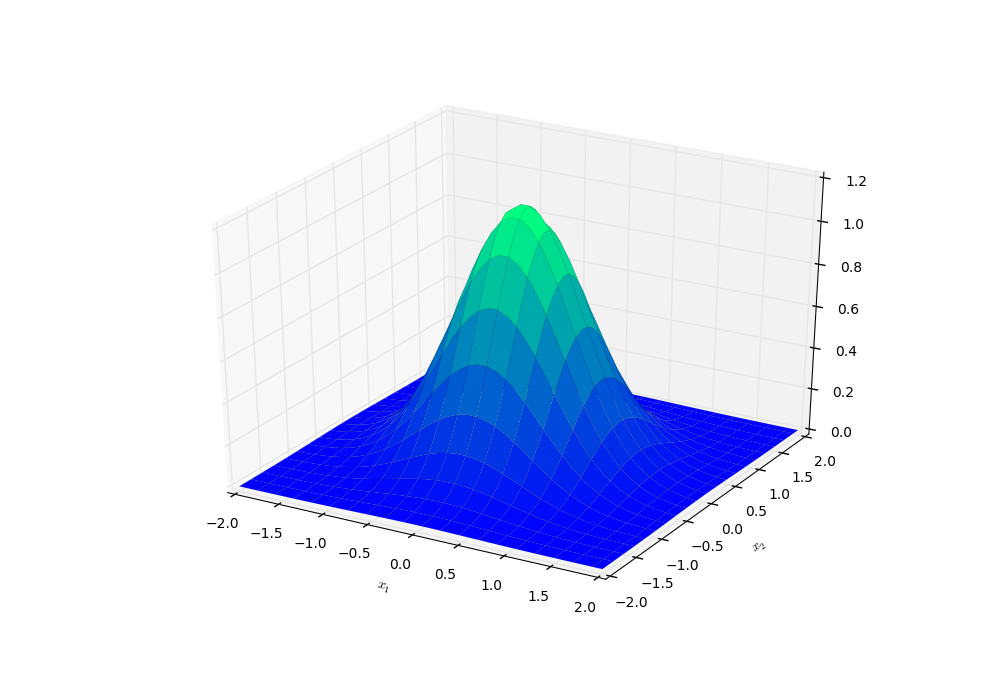
\includegraphics[width=0.88\textwidth]{std_iso_gaussian.png}\vspace{-1cm}
   			\caption{\vspace{-0.1cm} Isotropic 2D Gaussian $y = 3 \cdot \mathcal{N}(\boldsymbol{x} \big\vert \boldsymbol{0}, \frac{2}{5} \boldsymbol{I}_2)$.}\vspace{-0.2cm}
  		\end{figure}
	\item \begin{figure}[h]
   			\centering
   			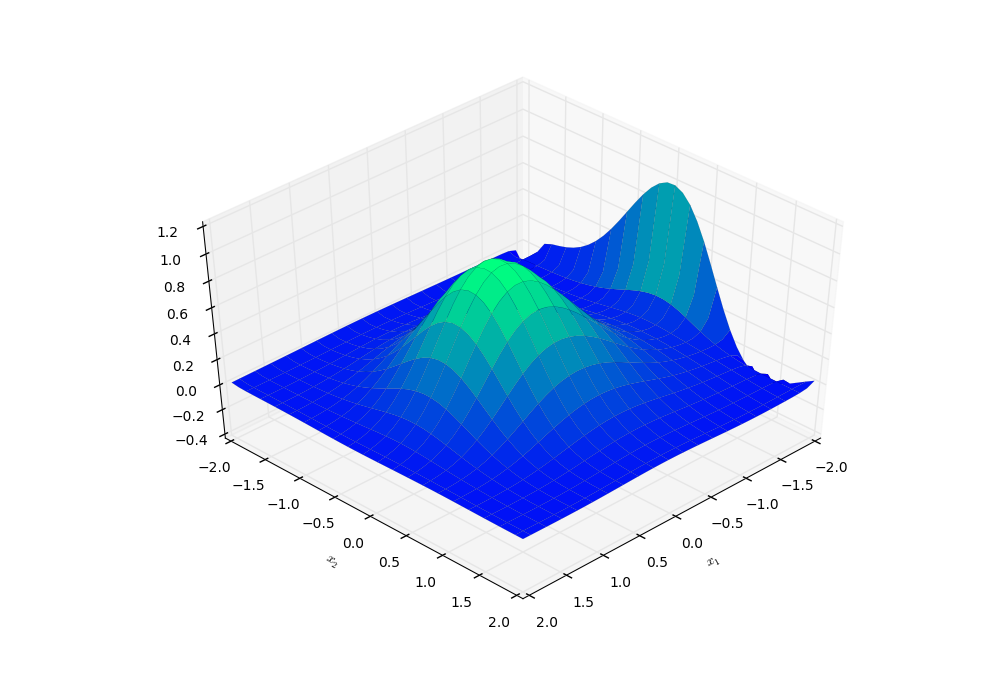
\includegraphics[width=0.88\textwidth]{ex2_2.png}\vspace{-1cm}
   			\caption{\vspace{-0.1cm} 2D graph of initial output of network.}\vspace{-0.2cm}
  		\end{figure}
	\item 
\end{enumerate}

%\vfill

\section{EM and doping}
\begin{enumerate}
	\item 
\end{enumerate}

%\vfill

\section{Handwritten digit recognition}
\begin{enumerate}
	\item
\end{enumerate}

\end{document}